\chapter{Návrh aplikace}

Tato kapitola se zabývá návrhem mobilní aplikace na základě výsledků provedené analýzy.
Cílem návrhu je definovat funkční rozsah aplikace, její strukturu, uživatelské rozhraní a technologické řešení tak, aby odpovídaly potřebám cílových uživatelů a zvolenému zaměření aplikace.
K~tomuto byly využity standardní techniky softwarového inženýrství.

Kapitola postupně představuje specifikaci funkčních a nefunkčních požadavků, návrhové diagramy a návrh uživatelského rozhraní.
Závěrem je zdůvodněna volba použitých technologií, které tvoří základ implementace aplikace.


\section{Specifikace požadavků}

Tato kapitola specifikuje požadavky na navrhovanou mobilní aplikaci.
Požadavky vymezují očekávané chování systému a jeho kvalitativní vlastnosti z~pohledu uživatelů i provozu aplikace.
Specifikace tvoří základ pro návrh architektury a implementaci aplikace.

\subsection{Funkční požadavky}

Funkční požadavky definují služby a funkce, které systém poskytuje svým uživatelům.
Aplikace rozlišuje dva základní typy uživatelů: běžné návštěvníky aplikace a registrované uživatele.

\begin{itemize}
    \item Prohlížení a vyhledávání obchodů
    \begin{itemize}
        \item Systém umožňuje zobrazit obchody v~mapovém nebo seznamovém zobrazení.
        \item Systém umožňuje filtrovat obchody podle kategorie, maximální vzdálenosti od aktuální polohy a minimálního průměrného hodnocení.
        \item Systém umožňuje zobrazit detail obchodu, včetně popisu, fotografií, nabídky produktů, otevírací doby a kontaktních údajů.
    \end{itemize}

    \item Správa uživatelského účtu
    \begin{itemize}
        \item Systém umožňuje vytvoření uživatelského účtu.
        \item Systém umožňuje přihlášení a odhlášení uživatele.
        \item Systém umožňuje registrovanému uživateli upravovat své osobní a kontaktní údaje.
    \end{itemize}

    \item Správa obchodů
    \begin{itemize}
        \item Systém umožňuje registrovanému uživateli vytvářet nové obchody.
        \item Systém umožňuje registrovanému uživateli upravovat a odstraňovat obchody, jejichž je vlastníkem.
        \item Systém umožňuje registrovanému uživateli přidávat a upravovat u~svých obchodů název, popis, kategorie obchodu, fotografie, nabídku produktů a otevírací dobu.
    \end{itemize}

    \item Recenze
    \begin{itemize}
        \item Systém umožňuje registrovanému uživateli vytvářet recenze obchodů jiných uživatelů.
    \end{itemize}
\end{itemize}

Aplikace neslouží jako e-shop a neumožňuje přímý nákup ani vytváření objednávek.
Jejím cílem je poskytovat prostředek pro prezentaci nabídky domácích producentů a umožnit zájemcům snadno vyhledat obchody v~jejich okolí.

\subsection{Nefunkční požadavky}

Nefunkční požadavky popisují vlastnosti aplikace, které se netýkají přímo funkcionality, ale ovlivňují kvalitu, použitelnost a provoz aplikace.

\begin{itemize}
    \item Aplikace je implementována jako nativní mobilní aplikace pro platformu Android a využívá nativní API zařízení.
    \item Uživatelské rozhraní musí být přehledné, konzistentní a snadno použitelné i~pro méně technicky zdatné uživatele.
    \item Systém musí poskytovat dostatečnou odezvu uživatelského rozhraní při práci s~mapovým i seznamovým zobrazením obchodů a dalšími funkcemi aplikace.
    \item Přístup k~datům musí být omezen pouze na oprávněné uživatele prostřednictvím autentizace a řízení přístupových práv.
    \item Architektura aplikace musí umožňovat další rozšiřování funkcionality bez zásadních zásahů do existujícího kódu.
\end{itemize}


\section{Diagram případů užití}
Diagram případů užití (Use Case Diagram) slouží k~přehlednému znázornění základních funkcí aplikace a interakcí mezi uživateli a systémem.
Diagram vychází ze specifikace funkčních požadavků a zachycuje chování aplikace z~pohledu jednotlivých typů uživatelů.
Přehled aktérů a případů užití je znázorněn na obrázku~\ref{fig:use-case-diagram}.

V~rámci aplikace jsou rozlišeny tři základní role: obecný uživatel (User), zákazník (Customer) a prodejce (Seller).
Role zákazníka a prodejce jsou modelovány jako specializace obecného uživatele pomocí vztahu generalizace.
Společné případy užití jsou tak sdíleny všemi specializovanými rolemi.
Tyto specializované role jsou rozděleny podle toho, jakým způsobem chce uživatel aplikaci využívat a co je jeho cílem při používání aplikace.
Primárním cílem zákazníka je procházet obchody a jejich nabídku, zatímco primárním cílem prodejce je vytvářet a spravovat obchody a prezentovat svou nabídku zájemcům.

Obecný uživatel zahrnuje základní případy užití související s~registrací, přihlášením, odhlášením a úpravou uživatelského profilu.
Případ užití úpravy profilu je dále rozšířen o konkrétní podřízené případy užití (například aktualizace jména, profilového obrázku nebo kontaktních údajů).
Případy užití odhlášení a úpravy profilu jsou dostupné pouze přihlášeným uživatelům.

Zákazník může procházet obchody v~mapovém nebo seznamovém zobrazení, zobrazovat detail obchodu a filtrovat obchody podle kategorií, vzdálenosti nebo hodnocení.
Funkce filtrování obchodů je modelována pomocí vztahu \textit{<<extend>>}, kdy jednotlivé typy filtrů (podle kategorií, vzdálenosti nebo hodnocení) rozšiřují základní případ užití procházení obchodů.
Pokud je zákazník přihlášen, může vytvářet recenze obchodů ostatních uživatelů.

Role prodejce zahrnuje případy užití související se správou obchodů.
Případ užití správy obchodů je dále rozšířen o konkrétní operace, jako je aktualizace polohy, otevírací doby, správa nabídky produktů a kategorií.
Tyto případy užití jsou rovněž podmíněny přihlášením uživatele.

Případy užití vyžadující přihlášení jsou v diagramu označeny stereotypem <<requires login>>.

\begin{figure}[htbp]
    \centering
    \includegraphics[width=\textwidth]{res/use_case_diagram}
    \caption{Diagram případů užití aplikace}
    \label{fig:use-case-diagram}
\end{figure}
\FloatBarrier


\section{Diagram tříd}

Diagram tříd (anglicky Class Diagram) popisuje strukturu aplikace z~pohledu hlavních entit, jejich atributů a vztahů mezi nimi.
Diagram vychází ze specifikace funkčních požadavků a diagramu případů užití a slouží jako podklad pro návrh datového modelu a implementaci aplikační logiky.
Modeluje základní entity tak, aby systém mohl plnit požadované funkce a zajišťoval konzistenci dat.
Přehled hlavních tříd a jejich vztahů je znázorněn na obrázku~\ref{fig:class-diagram}.

\begin{figure}[p]
    \centering
    \includegraphics[width=\textwidth]{res/class_diagram}
    \caption{Diagram tříd aplikace}
    \label{fig:class-diagram}
\end{figure}

\subsection{Entita uživatele}
Jednou ze základních entit je uživatel (User), který reprezentuje registrovaného uživatele aplikace.
Uživatel je identifikován jednoznačným identifikátorem a obsahuje základní osobní údaje, profilový obrázek a kontaktní informace.
Identifikátor je typu UUID, což zajišťuje jeho jedinečnost napříč celým systémem.
Kontaktní údaje jsou modelovány samostatnou třídou \texttt{Contact\-Info}, která je s~uživatelem svázána kompozicí, jelikož bez existence uživatele nemají samostatný význam.
Profilový obrázek je volitelný a je reprezentován hodnotovým objektem \texttt{Image\-Resource}, který uchovává odkaz na externě uložený obrazový soubor.

\subsection{Entita obchodu}
Druhou klíčovou entitou je obchod (Shop), který reprezentuje obchod vytvořený registrovaným uživatelem, kde může nabízet své produkty.
Obchod je také identifikován jednoznačným identifikátorem typu UUID\@.
Obchod obsahuje atributy: id, název, popis, vlastník, seznam kategorií, obrázky, nabídku produktů, polohu a otevírací dobu.
Základní atributy jako název a popis jsou oba typu \texttt{String} a popis je volitelný.

Obchod je svázán s~uživatelem prostřednictvím asociace, která vyjadřuje vlastnictví obchodu konkrétním uživatelem.

Kategorie obchodu je reprezentována hodnotovým objektem typu \texttt{Shop\-Category}, který obsahuje název kategorie a barvu pro vizuální odlišení.
Vztah mezi obchodem a kategoriemi je modelován jako kompozice, protože kategorie jsou vlastněny konkrétním obchodem.
Oproti možnosti modelovat kategorie jako samostatné entity sdílené mezi obchody poskytuje tento přístup větší flexibilitu jak při volbě názvu kategorie, tak i při volbě její barvy.
Uživatel si tak může zvolit libovolnou kombinaci názvu a barvy kategorie.
Požadované filtrování obchodů podle kategorií bude realizováno pomocí normalizovaných názvů kategorií ze všech obchodů.

Obrázky obchodu jsou reprezentovány jako seznam již zmiňovaných hodnotových objektů \texttt{Image\-Resource}.

Nabídka produktů je modelována hodnotovým objektem \texttt{Menu}, který obsahuje seznam položek nabídky typu \texttt{Menu\-Item}.
Každá položka nabídky obsahuje název, volitelný popis, cenu a informaci o~dostupnosti.
Cena je reprezentována hodnotovým objektem \texttt{Price\-Label}, který uchovává cenu jako řetězec.
Uživatel tak může cenu popsat vzhledem k~měně a jednotce v~jaké se produkt nabízí (například \enquote{150 Kč / kg}).
Vzhledem k tomu, že aplikace neslouží k přímému nákupu ani k provádění filtrování či řazení podle ceny produktů, je cena modelována jako textový údaj určený pouze k informační prezentaci nabídky.

Otevírací doba obchodu je reprezentována rozhraním \texttt{Opening\-Hours}, které má dvě implementace: \texttt{Time\-Opening\-Hours} a \texttt{Message\-Opening\-Hours}.
První implementace uchovává otevírací dobu jako mapu dnů v~týdnu na otevírací hodiny v~případě, že producent je dostupný v~pravidelných časech.
Druhá implementace uchovává otevírací dobu jako volitelnou zprávu v~případě, že producent chce například uvést, aby ho zájemce nejdříve kontaktoval.

Poloha obchodu je modelována hodnotovým objektem \texttt{Location}, který obsahuje zeměpisnou šířku a délku jako desetinná čísla.

\subsection{Entita recenze}
Poslední entitou je recenze (Review), která reprezentuje hodnocení obchodu uživatelem.
Recenze je identifikována jednoznačným identifikátorem typu UUID a obsahuje atributy: id, autor, obchod, hodnocení a volitelný komentář.
Recenze je svázána s~uživatelem prostřednictvím asociace, která vyjadřuje autora recenze.
S~obchodem je recenze rovněž svázána asociací, jelikož recenze reprezentuje interakci mezi uživatelem a konkrétním obchodem, nikoli vnitřní součást těchto entit.
Přestože recenze bez existence obchodu ztrácí svůj praktický význam, není modelována jako kompozitní součást obchodu, protože má vlastní identitu a samostatný životní cyklus.


\section{Návrh uživatelského rozhraní}
% TODO: Jak a na kolika různých lidech plánujete testovat kvalitu UI?
Návrh uživatelského rozhraní (UI) se zaměřuje na vytvoření přehledného a intuitivního prostředí pro uživatele aplikace.
Cílem je zajistit, aby uživatelé mohli snadno a efektivně využívat funkce aplikace a dosahovat svých cílů, které vychází z~funkčních požadavků a diagramu případů užití.
Návrh UI zahrnuje rozvržení obrazovek, navigační strukturu a interakční prvky.
Při návrhu rozhraní je kladen důraz na konzistenci ovládacích prvků, díky čemuž se uživatel snadno zorientuje v~aplikaci, jasnou navigaci aplikací a minimalizaci počtu kroků potřebných k~provedení akcí.

\subsection{Barevné schéma}
Při návrhu byly využity principy Material Designu, které zajišťují jednotný a moderní vzhled aplikace.
Material Design je designový systém vyvinutý společností Google, který poskytuje sadu doporučených postupů a komponent pro tvorbu uživatelských rozhraní.\footfullcite{material_design}

Barevná paleta byla vygenerována pomocí nástroje Material Theme Builder, který generuje barevné schéma v~souladu s~principy Material Designu.\footfullcite{material_theme_builder}
Po zadání primární barvy do nástroje nám vytvoří kompletní sadu barev pro světlé i tmavé téma aplikace.
V~případě potřeby lze barvy dále upravovat, avšak pro základní návrh zajišťují tyto vygenerované barvy konzistentní a esteticky příjemný vzhled aplikace.
Pro primární barvu byla zvolena tmavě zelená (\#3C6838), která evokuje přírodní potraviny a zemědělství.
Ostatní barvy byly nástrojem Material Theme Builder vygenerovány na základě této primární barvy, aby se vzájemně doplňovaly.
Zajišťují tak dostatečný kontrast pro čitelnost textu a vizuální přitažlivost aplikace.

Významnou barvou v~Material Design paletě je barva \textit{surface}, která je používána jako pozadí pro většinu obrazovek aplikace (v~obrázku~\ref{fig:color-palette} je použita jako pozadí boxu \enquote{Světlý motiv}, respektive \enquote{Tmavý motiv}).
Těmi nejdůležitějšími barvami jsou ale barvy primární, sekundární, terciární a jejich kontejnerové varianty (zobrazeny na~obrázku~\ref{fig:color-palette}).
Primární, sekundární a terciární barvy jsou používány pro zvýraznění důležitých prvků uživatelského rozhraní, jako jsou tlačítka, ikony a další interakční prvky.
Kontejnerové varianty těchto barev jsou používány pro větší plochy, které jsou třeba zvýraznit, jako jsou karty nebo větší tlačítka.\footfullcite{material3_color_roles}

\begin{figure}[htbp]
    \centering
    \includegraphics[width=\textwidth]{res/color_palette}
    \caption{Barevná paleta aplikace}
    \label{fig:color-palette}
\end{figure}

\subsection{Rozvržení obrazovek}
Návrh rozvržení obrazovek aplikace vychází z~funkčních požadavků a diagramu případů užití.
Je důležité, aby uživatelské rozhraní bylo přehledné a intuitivní, což umožní uživatelům snadno najít a využít požadované funkce aplikace.

Ve spodní části základních obrazovek se nachází \textbf{navigační lišta} (obrázky~\ref{fig:ui-overview}), která obsahuje tři ikony představující tři hlavní obrazovky aplikace: \enquote{Moje obchody}, \enquote{Úvodní obrazovka} a \enquote{Profil uživatele}.
Díky ní může uživatel snadno navigovat mezi právě těmito základními obrazovkami aplikace.
První ikona v~liště slouží pro navigaci na obrazovku se seznamem obchodů vytvořených uživatelem.
Tato ikona se v~navigační liště zobrazuje pouze pokud je uživatel přihlášen.
Druhá ikona slouží pro navigaci na úvodní obrazovku s~mapovým a seznamovým zobrazením obchodů.
Třetí ikona slouží pro navigaci na obrazovku profilu uživatele.
V~případě, že je uživatel přihlášen, je na této obrazovce možné upravit osobní údaje.
V~opačném případě se zobrazí přihlašovací obrazovka, kde se může uživatel přihlásit nebo zaregistrovat nový účet.

\textbf{Úvodní obrazovkou} aplikace je obrazovka, kde uživatel může zvolit mezi mapovým a seznamovým zobrazením obchodů.

Výchozím zobrazením je mapové zobrazení, kde mapa ukazuje polohu uživatele a okolní obchody jako značky na mapě (obrázek~\ref{fig:map-view}).
Při kliknutí na značku obchodu se zobrazí detail obchodu jako spodní panel, který obsahuje detaily obchodu (obrázek~\ref{fig:map-view-shop-detail}).

V~seznamovém zobrazení jsou obchody zobrazeny jako karty v~seznamu, které obsahují pouze základní informace o~obchodu, aby byly karty přehledné, ale zároveň obchod dostatečně popisovaly (obrázek~\ref{fig:list-view}).
Zde se při kliknutí na kartu obchodu zobrazí detail obchodu na samostatné obrazovce (obrázek~\ref{fig:shop-detail}).

Obě zobrazení mají společnou spodní nabídku, kde může uživatel přepínat mezi mapovým a seznamovým zobrazením a otevřít dialog pro filtry.
Při kliknutí na tlačítko filtrů se zobrazí dialog, kde může uživatel zvolit jaký filtr chce upravit (kategorie, vzdálenost, hodnocení) a následně nastavit jeho hodnoty (obrázek~\ref{fig:filters}).
V~záložce \enquote{Filtry kategorií} může uživatel přidat název kategorie, které chce zobrazit.
Názvy jsou doporučovány na základě jejich četnosti v~existujících obchodech, aby uživatel mohl snadno vybrat nejčastější kategorie a podle již zadaných počátečních písmen.
V~záložce \enquote{Filtr vzdálenosti} může uživatel zvolit maximální vzdálenost obchodů od své aktuální polohy pomocí posuvníku a v~záložce \enquote{Filtr hodnocení} může uživatel zvolit minimální průměrné hodnocení obchodů pomocí hvězdiček.

\begin{figure}[htbp]
    \centering

    \begin{subfigure}[t]{0.24\textwidth}
        \centering
        \includegraphics[width=\linewidth]{res/ui/map_view}
        \caption{Mapové zobrazení obchodů}
        \label{fig:map-view}
    \end{subfigure}\hfill
    \begin{subfigure}[t]{0.24\textwidth}
        \centering
        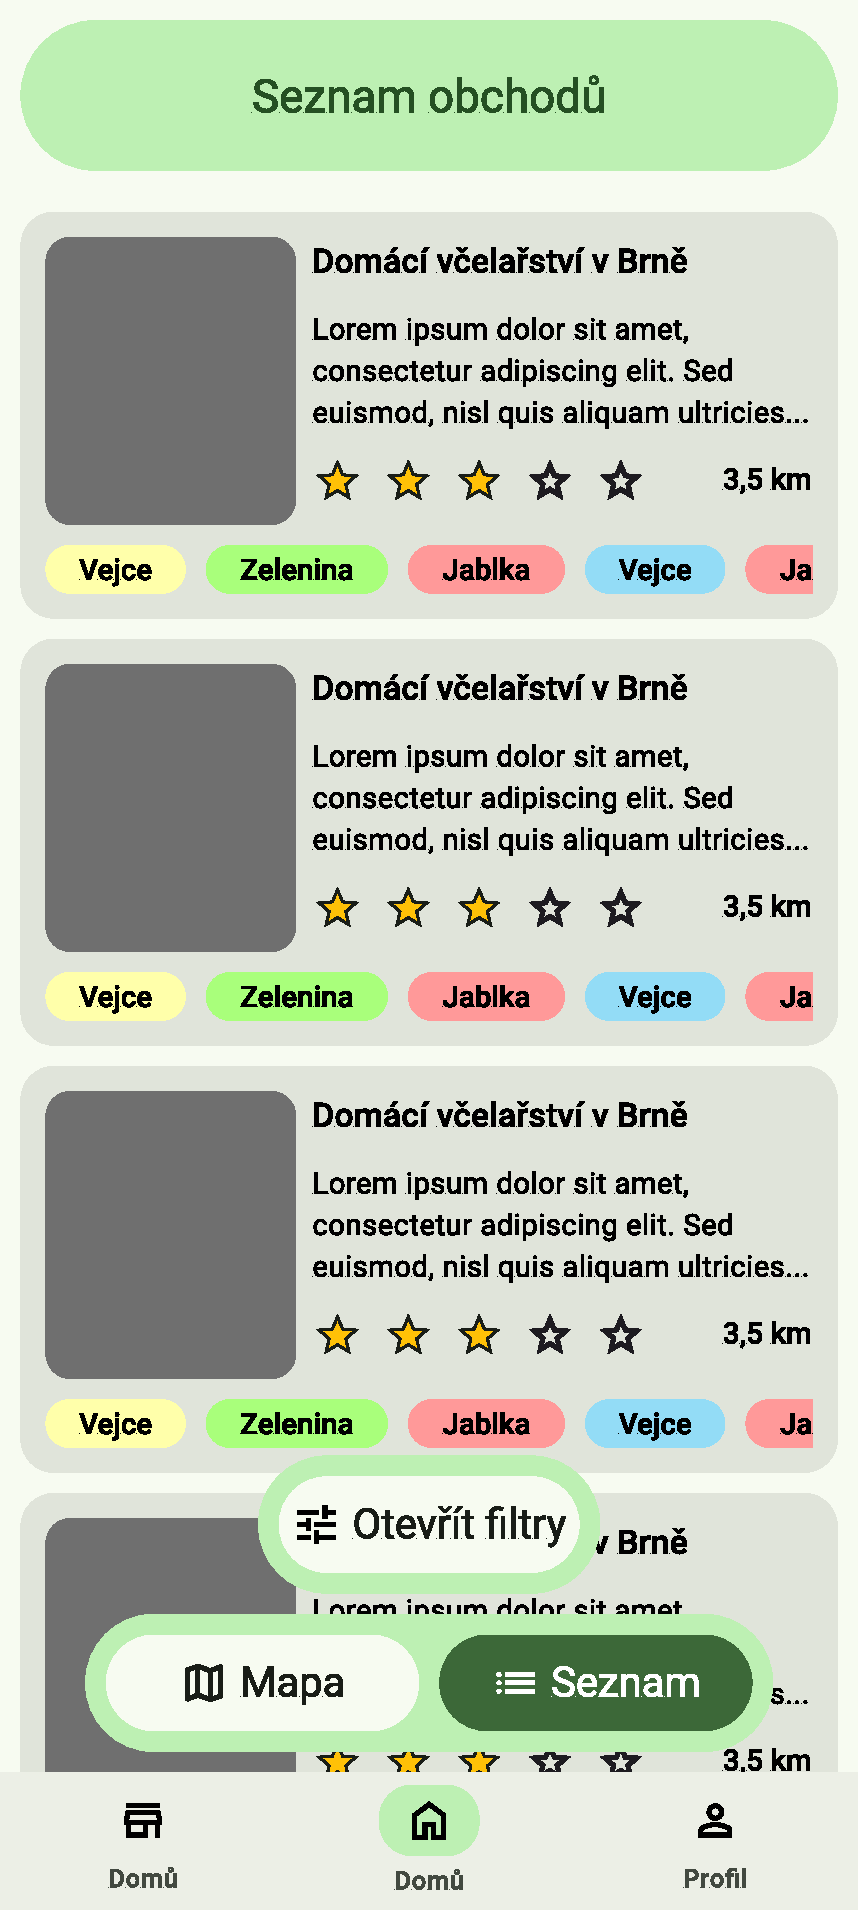
\includegraphics[width=\linewidth]{res/ui/list_view}
        \caption{Seznamové zobrazení obchodů}
        \label{fig:list-view}
    \end{subfigure}\hfill
    \begin{subfigure}[t]{0.24\textwidth}
        \centering
        \includegraphics[width=\linewidth]{res/ui/map_view_shop_detail}
        \caption{Detail obchodu v~mapovém zobrazení}
        \label{fig:map-view-shop-detail}
    \end{subfigure}\hfill
    \begin{subfigure}[t]{0.24\textwidth}
        \centering
        \includegraphics[width=\linewidth]{res/ui/shop_detail}
        \caption{Detail obchodu v~plném zobrazení}
        \label{fig:shop-detail}
    \end{subfigure}

    \caption{Přehled uživatelského rozhraní aplikace}
    \label{fig:ui-overview}
\end{figure}

\begin{figure}
    \captionsetup{size=small}
    \centering
    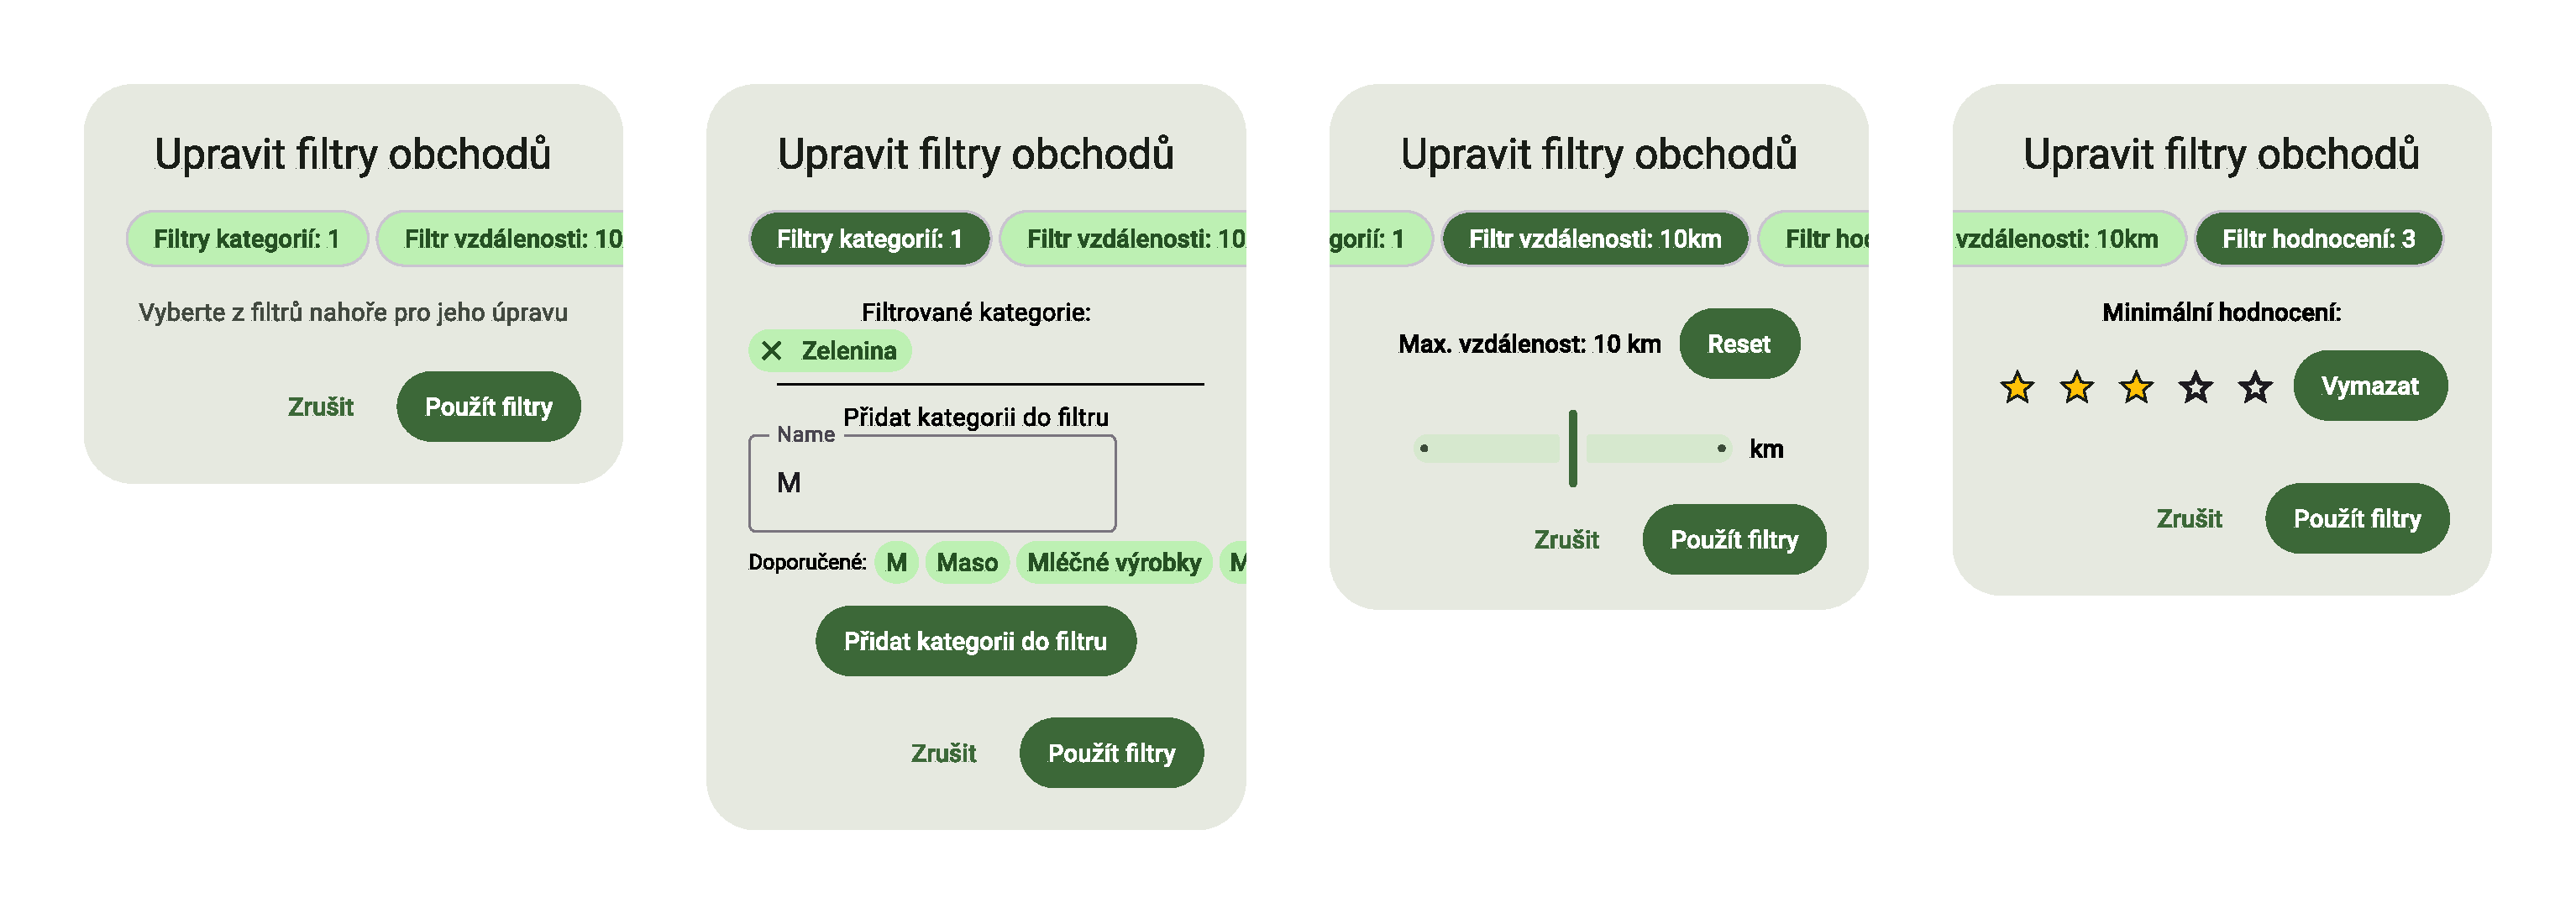
\includegraphics[width=\linewidth]{res/ui/filters}
    \caption{Dialog pro nastavení filtrů}
    \label{fig:filters}
\end{figure}

\textbf{Na obrazovce profilu} může uživatel upravit své osobní údaje, jak bylo specifikováno ve funkčních požadavcích.
Mezi tyto údaji patří jméno, kontaktní informace a profilový obrázek.
V~případě profilového obrázku může uživatel buď nahrát obrázek ze svého zařízení, nebo přímo vyfotit nový obrázek pomocí fotoaparátu zařízení.
Uživatel se zde také může odhlásit z~aplikace.

Na obrazovce \textbf{Moje obchody} má uživatel přehled o~všech obchodech, které vytvořil.
Obchody jsou zobrazeny jako karty v~seznamu, podobně jako v~seznamovém zobrazení na úvodní obrazovce.
Každá karta má však navíc tlačítka pro úpravu a odstranění obchodu.
Po kliknutí na tlačítko pro úpravu se spustí proces úpravy obchodu a po kliknutí na tlačítko pro odstranění se daný obchod smaže.
K~tomu se ve spodní části obrazovky nachází tlačítko pro vytvoření nového obchodu.
Po kliknutí na toto tlačítko se spustí proces vytváření nového obchodu.

\textbf{Proces vytváření a úpravy obchodu} je rozdělen do několika kroků a každý krok je zobrazen na samostatné obrazovce.
Uživatel může mezi těmito kroky libovolně navigovat pomocí dvou spodních tlačítek \enquote{Předchozí} a \enquote{Další}.

V~prvním kroku uživatel zadává název a polohu obchodu na mapě (obrázek~\ref{fig:create-shop-step-01}).
Jsou to kromě samotné nabídky nejvýznamnější údaje, které obchod popisují a kterých si zájemci všimnou jako první.

V~druhém kroku uživatel přidává fotografie a popis obchodu (obrázek~\ref{fig:create-shop-step-02}).
Pro fotografie má uživatel na výběr mezi přidáním ze svého zařízení nebo vyfocením nové fotografie pomocí fotoaparátu zařízení.
Fotografie může uživatel přidávat, mazat nebo měnit jejich pořadí.
Pro popis obchodu je k~dispozici textové pole, kde uživatel může zadat libovolný dlouhý text.

Ve třetím kroku uživatel přidává kategorie obchodu a položky nabídky (obrázek~\ref{fig:create-shop-step-03}).
Kategorie jsou reprezentovány názvem a barvou, kterou si uživatel může zvolit z~předdefinované palety barev (obrázek~\ref{fig:create-shop-add-edit-category}).
Názvy kategorií se uživatelovi doporučují na základě jejich četnosti v~existujících obchodech, aby uživatel mohl snadno vybrat nejpopulárnější kategorie a jeho obchod byl tak lépe dohledatelný.
Položky nabídky produktů (Menu produktů) obsahují název, volitelný popis, cenu a informaci o~dostupnosti (obrázek~\ref{fig:create-shop-add-edit-product}).
Po kliknutí na tlačítko \enquote{Přidat produkt} se zobrazí dialog pro zadání těchto údajů o~nové položce nabídky.
Každá položka nabídky je zobrazena jako karta v~seznamu a kromě zobrazení údajů obsahuje také tlačítka pro úpravu a odstranění položky nabídky.

Ve čtvrtém kroku uživatel zadává otevírací dobu obchodu (obrázek~\ref{fig:create-shop-step-04}).
Uživatel má na výběr mezi dvěma způsoby zadání otevírací doby: jako pravidelnou denní otevírací dobu (obrázek~\ref{fig:create-shop-opening-hours-time}), kde může uživatel ke každému dni v~týdnu zadat zprávu, kde popíše otevírací hodiny (například \enquote{9:00-11:00, 13:00-17:00}), nebo jako volitelnou zprávu, kde uživatel může zadat libovolný text (například \enquote{Kontaktujte mě předem telefonicky}).

Posledním krokem je shrnutí, kde může uživatel zkontrolovat všechny zadané údaje před vytvořením nebo úpravou obchodu.
Tato obrazovka je téměř totožná jako obrazovka detailu obchodu, ale obsahuje navíc tlačítka \enquote{Předchozí} a \enquote{Potvrdit} (místo tlačítka \enquote{Další} jako v~předchozích krocích).

\begin{figure}[htbp]

    \centering
    \begin{subfigure}[t]{0.24\textwidth}
        \centering
        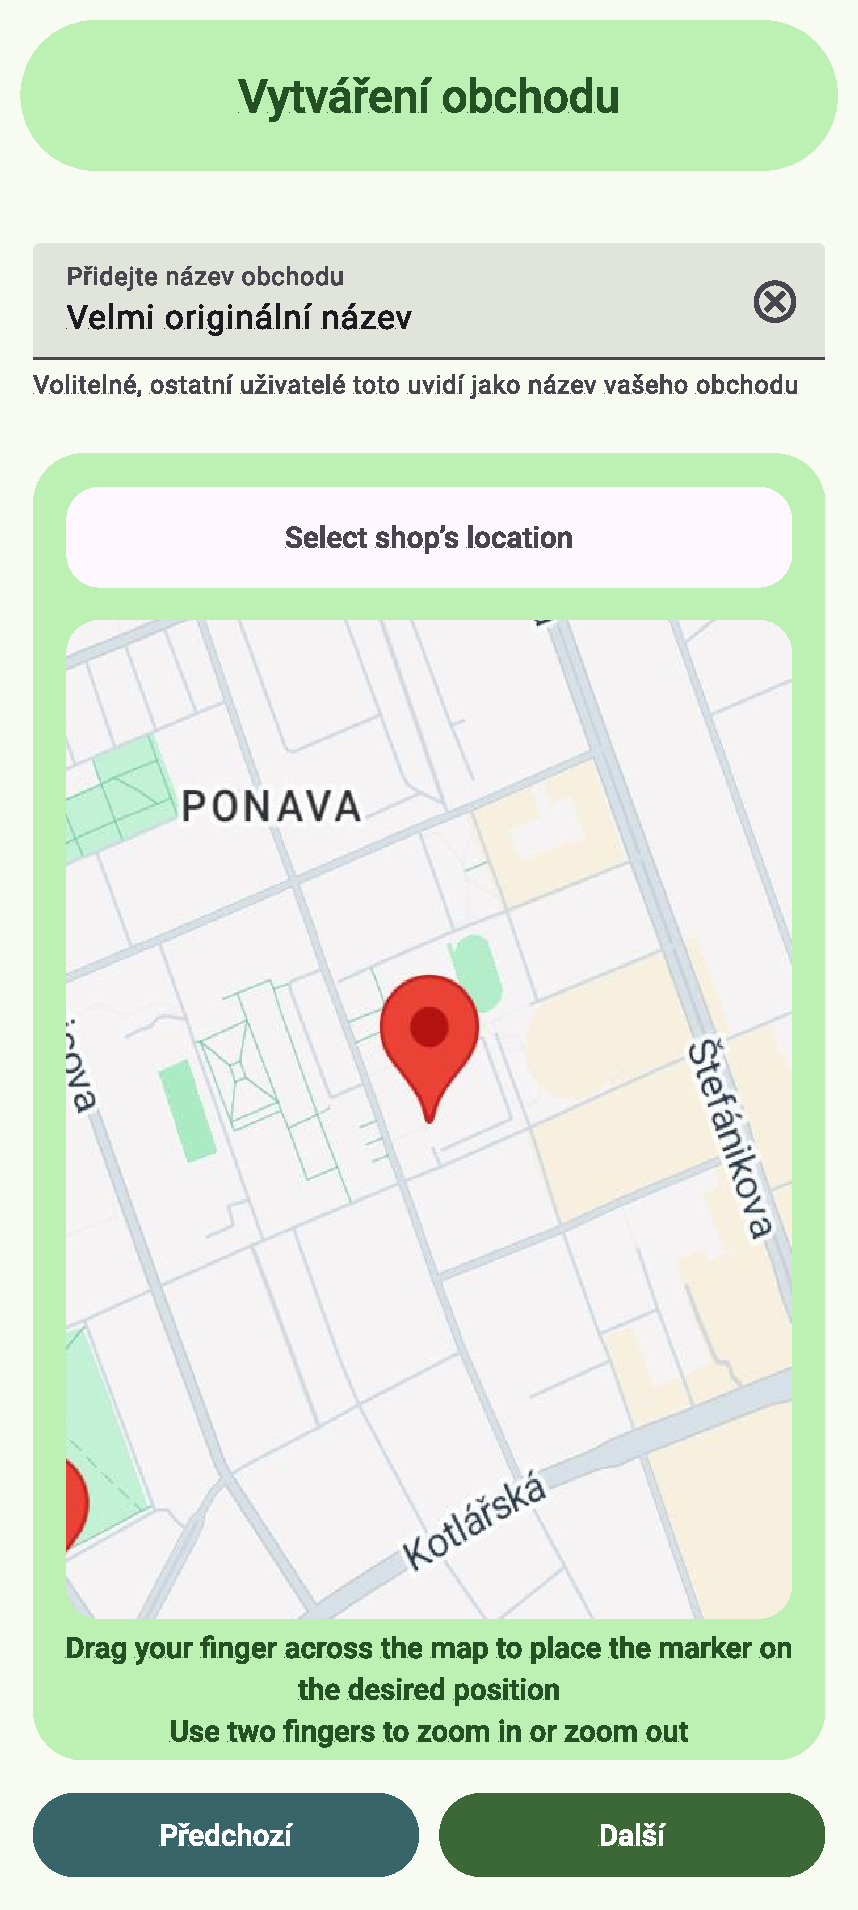
\includegraphics[width=\linewidth]{res/ui/create_flow/create_shop_01}
        \caption{Krok 1: Název a poloha obchodu}
        \label{fig:create-shop-step-01}
    \end{subfigure}\hfill
    \begin{subfigure}[t]{0.24\textwidth}
        \centering
        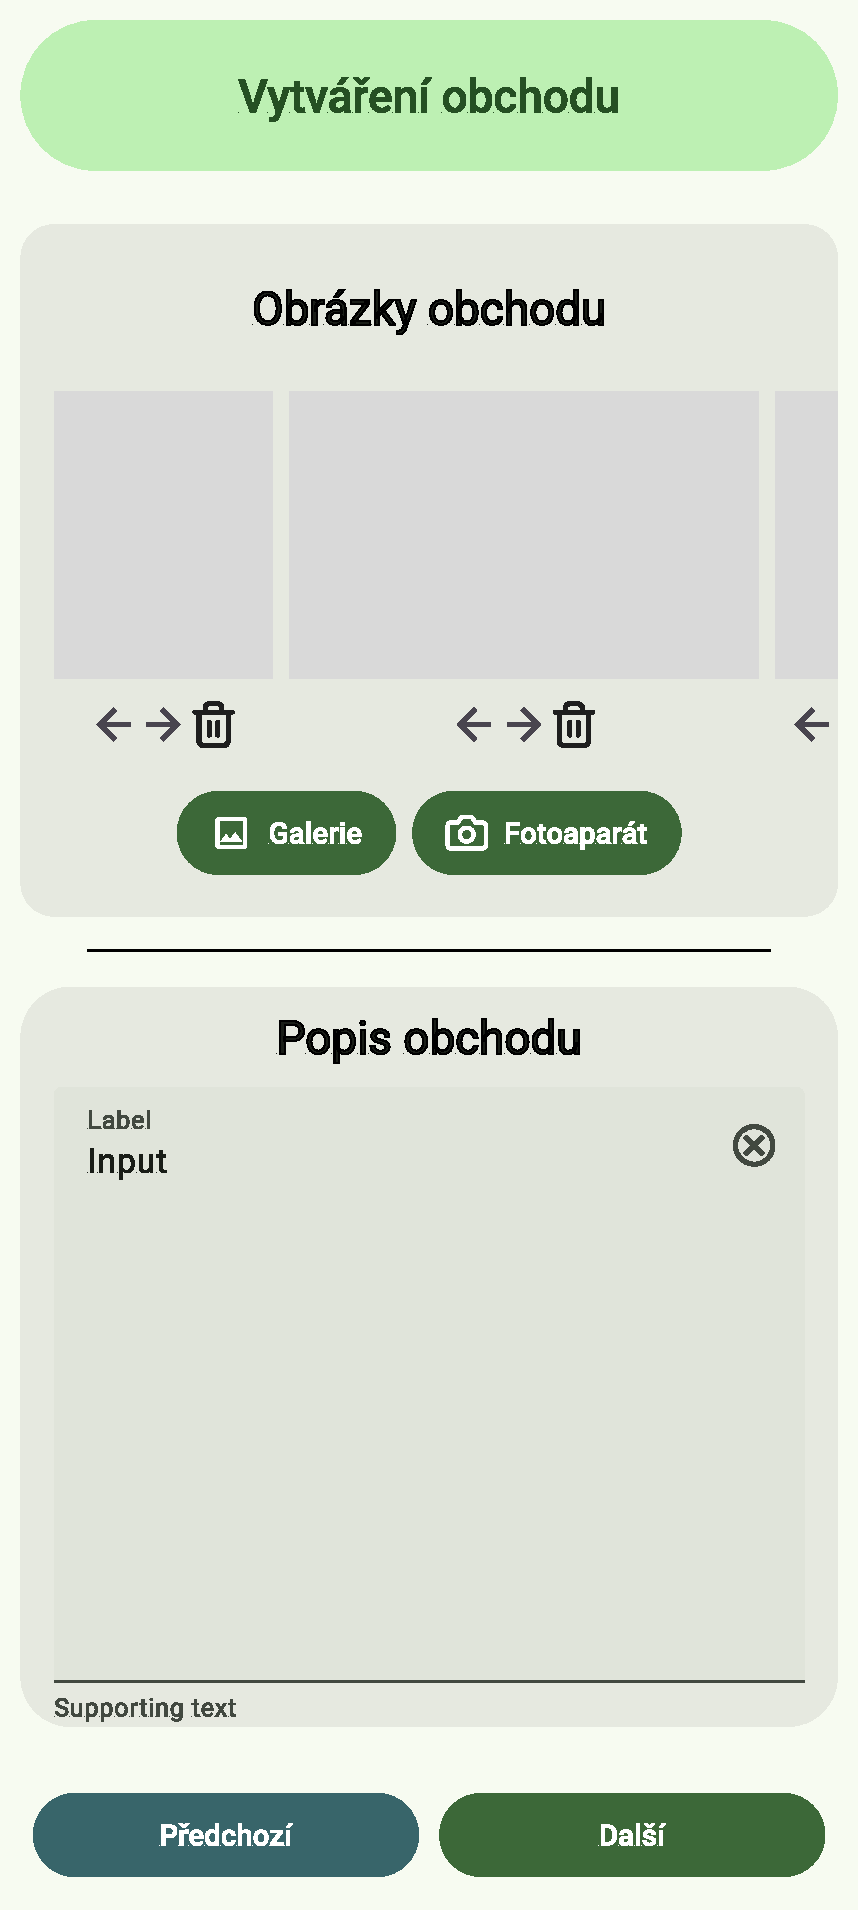
\includegraphics[width=\linewidth]{res/ui/create_flow/create_shop_02}
        \caption{Krok 2: Obrázky a popis obchodu}
        \label{fig:create-shop-step-02}
    \end{subfigure}\hfill
    \begin{subfigure}[t]{0.24\textwidth}
        \centering
        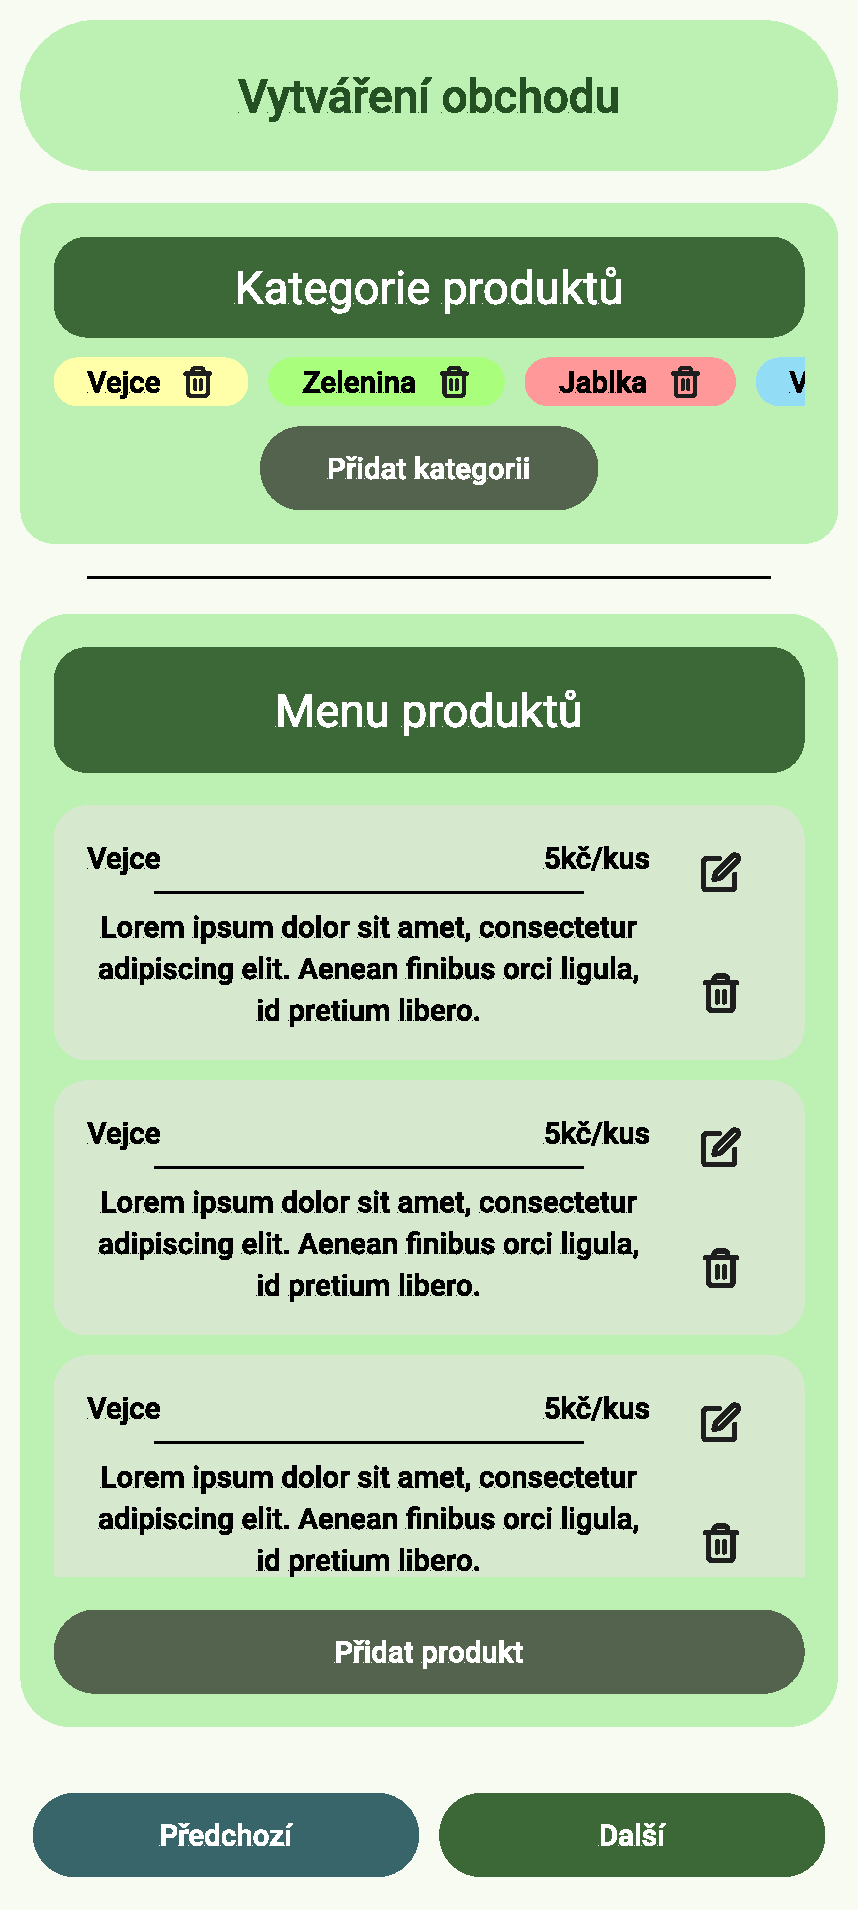
\includegraphics[width=\linewidth]{res/ui/create_flow/create_shop_03}
        \caption{Krok 3: Kategorie obchodu a nabídka produktů}
        \label{fig:create-shop-step-03}
    \end{subfigure}\hfill
    \begin{subfigure}[t]{0.24\textwidth}
        \centering
        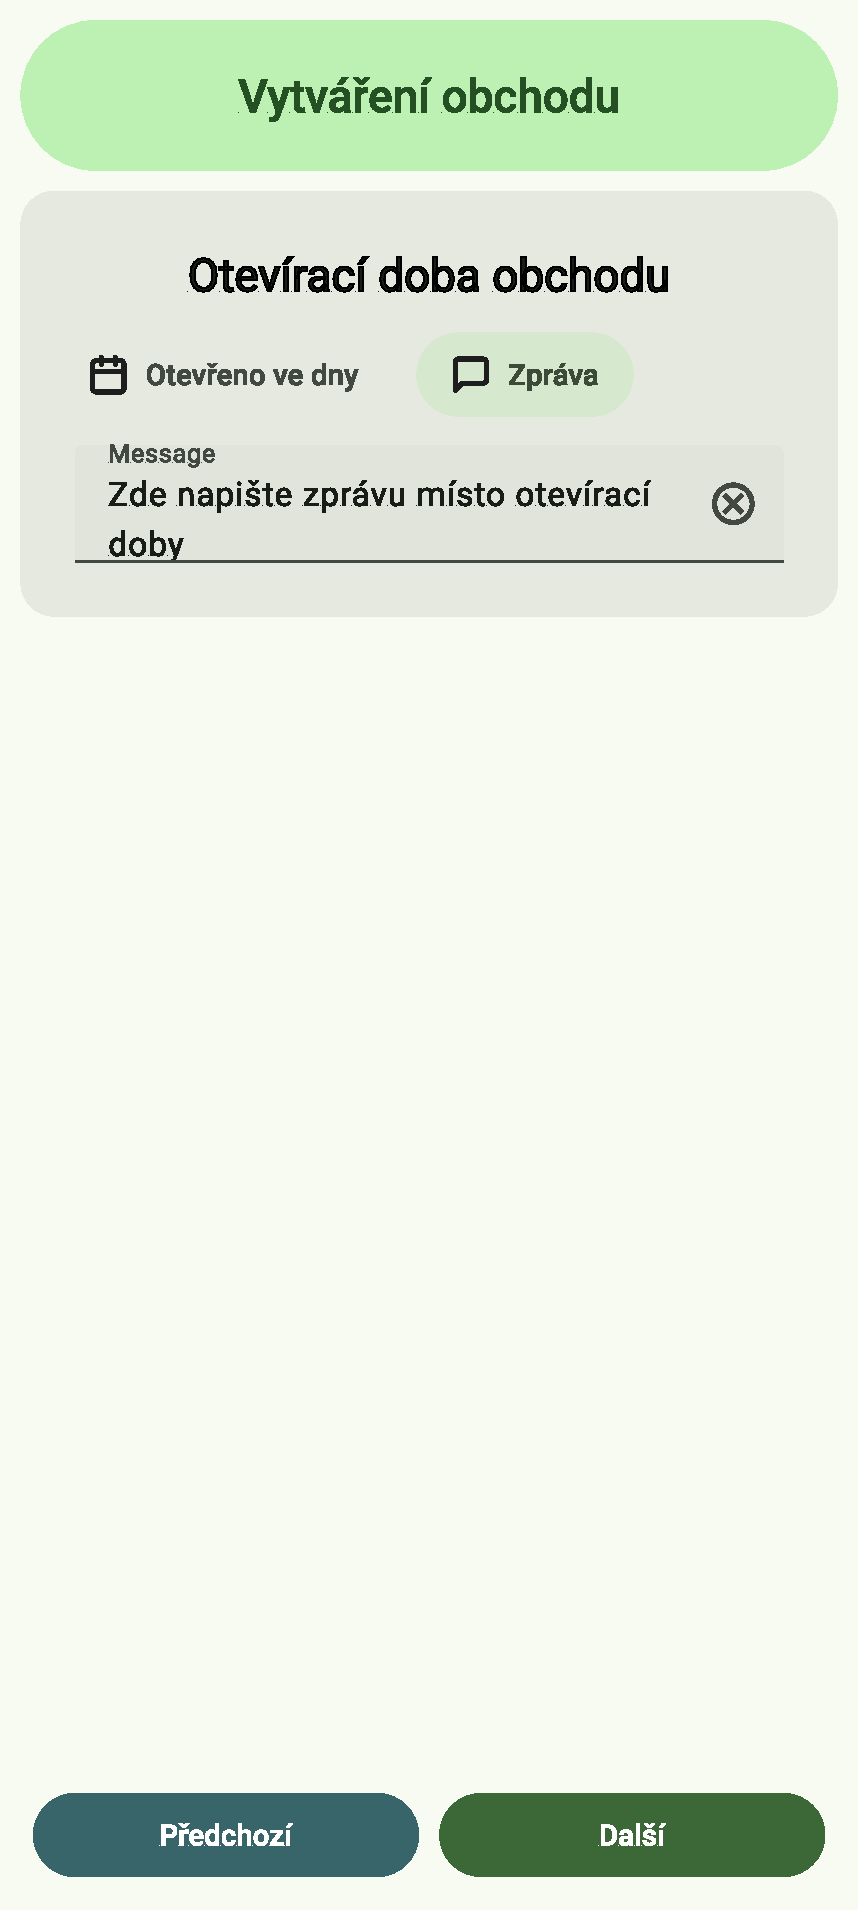
\includegraphics[width=\linewidth]{res/ui/create_flow/create_shop_04}
        \caption{Krok 4: Otevírací doba obchodu – zpráva}
        \label{fig:create-shop-step-04}
    \end{subfigure}

    \caption{Kroky vytváření a úpravy obchodu}
    \label{fig:create-shop-steps}
\end{figure}

\begin{figure}[htbp]
    \centering
    \begin{subfigure}[t]{0.24\textwidth}
        \centering
        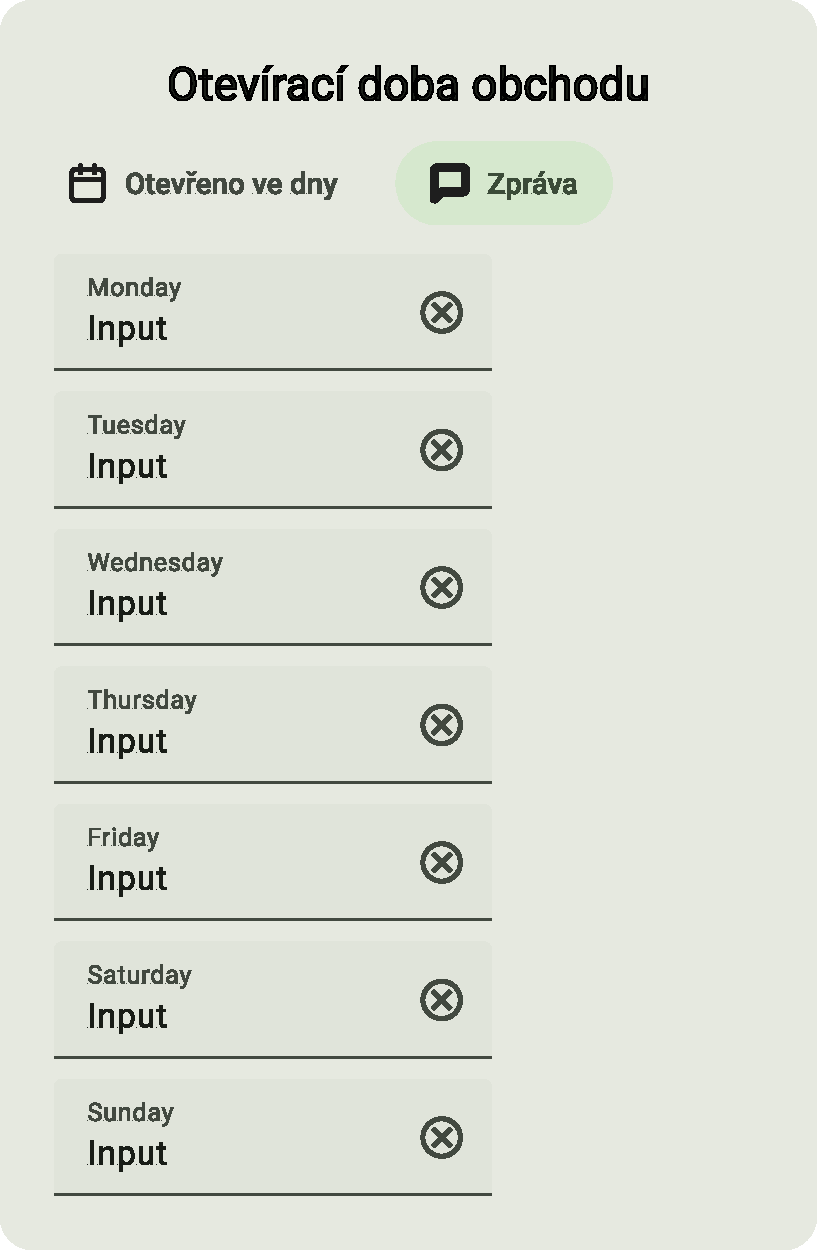
\includegraphics[width=\linewidth]{res/ui/create_flow/opening_hours_time}
        \caption{Denní otevírací doba obchodu}
        \label{fig:create-shop-opening-hours-time}
    \end{subfigure}
    \hspace{0.02\textwidth}
    \begin{subfigure}[t]{0.24\textwidth}
        \centering
        \includegraphics[width=\linewidth]{res/ui/create_flow/add/edit_category}
        \caption{Přidání / úprava kategorie obchodu}
        \label{fig:create-shop-add-edit-category}
    \end{subfigure}
    \hspace{0.02\textwidth}
    \begin{subfigure}[t]{0.24\textwidth}
        \centering
        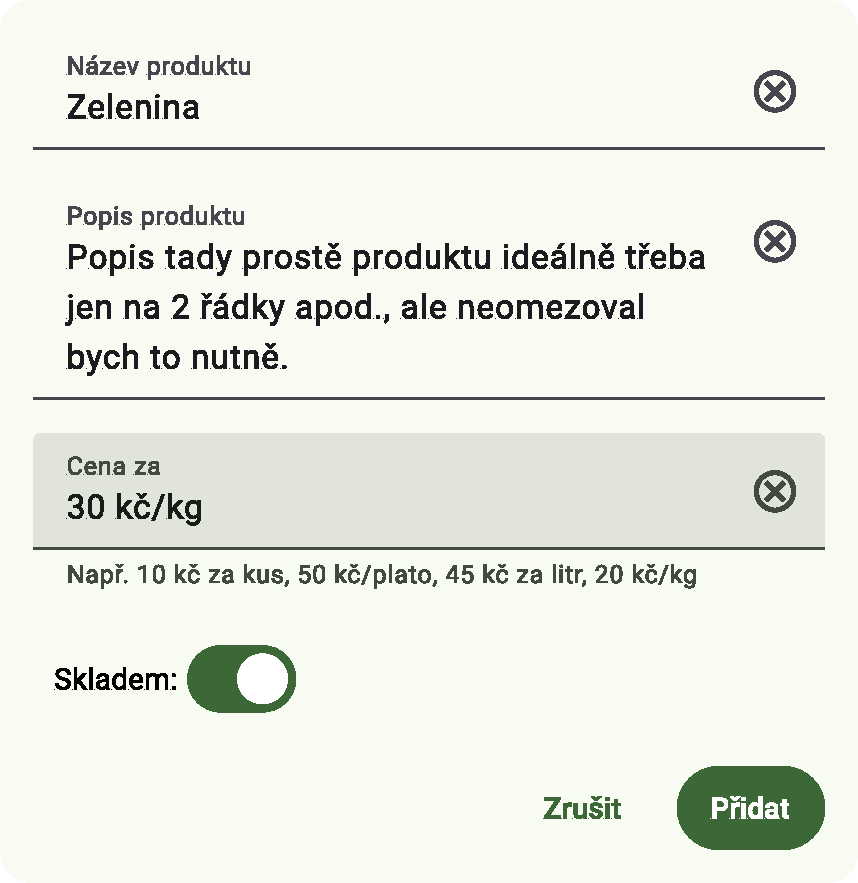
\includegraphics[width=\linewidth]{res/ui/create_flow/add/edit_product}
        \caption{Přidání / úprava položky nabídky obchodu}
        \label{fig:create-shop-add-edit-product}
    \end{subfigure}

    \caption{Dodatečné prvky vytváření a úpravy obchodu}
    \label{fig:create-shop-additional}
\end{figure}


\section{Výběr technologií}
Volba použitých technologií vychází z~požadavků aplikace a zohledňuje faktory jako je efektivita vývoje, uživatelský zážitek, škálovatelnost a údržba aplikace.
Cílem je zvolit technologie vhodné pro vytvoření funkční, spolehlivé a uživatelsky přívětivé aplikace, která bude odpovídat potřebám cílových uživatelů a splňovat stanovené požadavky.

\subsection{Volba cílové platformy}
Při volbě platformy pro vývoj aplikace se obvykle nabízejí tři hlavní možnosti: mobilní aplikace, webová aplikace a desktopová aplikace.
Navrhovaná aplikace využívá funkce, jako jsou fotoaparát zařízení, galerie obrázků, zjišťování aktuální polohy uživatele a mapové zobrazení okolí.
Aplikace je navržena tak, aby byla využitelná i mimo domov, například při cestování nebo návratu z~cesty, kdy uživatel potřebuje rychle vyhledat obchody v~okolí své aktuální polohy.
Zároveň obchody v~aplikaci poskytují zájemcům kontaktní údaje na producenty, aby je mohli snadno kontaktovat například formou telefonního hovoru, SMS nebo odkazem na sociální sítě.
V~praxi k~této interakci uživatelé ve většině případů využívají mobilní telefon, takže i zde je vhodnější mít aplikaci přímo na mobilním zařízení.
Z~uvedených důvodů je nejvhodnější aplikační platformou mobilní aplikace.
Webová aplikace by sice zajistila vyšší míru dostupnosti napříč zařízeními, avšak v~prostředí mobilních zařízení by ve srovnání s~nativní mobilní aplikací poskytovala méně vhodný uživatelský zážitek, jak z~hlediska výkonu, odezvy a použitelnosti, tak i z~hlediska přístupu k~nativním funkcím zařízení.
V~České republice je nejrozšířenějším operačním systémem pro mobilní zařízení Android, a proto byla jako cílová platforma zvolena mobilní aplikace pro platformu Android.\footfullcite{android_market_share_cz}

Alternativou k~nativnímu vývoji by bylo využití multiplatformních frameworků, jako jsou Flutter nebo React Native, které umožňují cílit na více platforem z~jednoho kódu.
Tato řešení však přinášejí další vrstvu abstrakce a zvyšují složitost integrace s~nativními funkcemi zařízení, jako jsou práce s~mapami, polohou uživatele nebo fotoaparátem.\footfullcite{native_vs_cross_platform}
Vzhledem k~zaměření práce výhradně na platformu Android, rozsahu bakalářské práce a důrazu na návrh uživatelského rozhraní, aplikační logiky a využití nativních funkcí zařízení bylo zvoleno \textbf{nativní řešení pro platformu Android}.

\subsection{Programovací jazyk a UI framework}

Pro vývoj mobilní aplikace pro platformu Android bylo nutné zvolit vhodný programovací jazyk a framework pro tvorbu uživatelského rozhraní.
V~současnosti patří mezi nejčastěji používané kombinace pro vývoj nativních Android aplikací Java s~XML, Kotlin s~XML a Kotlin s~frameworkem Jetpack Compose.\footfullcite{compose_vs_xml, kotlin_vs_java_android}

Jako programovací jazyk byl zvolen Kotlin, který je moderním a oficiálně doporučovaným jazykem pro vývoj Android aplikací.
Ve srovnání s~jazykem Java nabízí Kotlin kratší a čitelnější syntaxi, lepší podporu moderních programovacích paradigmat a vyšší bezpečnost typů díky práci s~nulovatelností (null-safety).

Pro tvorbu uživatelského rozhraní byl zvolen framework Jetpack Compose, který umožňuje deklarativní přístup k~návrhu UI\@.
Tento přístup snižuje množství potřebného kódu, usnadňuje jeho údržbu a zrychluje vývoj aplikace.
Jetpack Compose je navíc přirozeně integrován se správou stavu aplikace, což usnadňuje práci s~dynamickým obsahem a uživatelskými interakcemi.

Zvolená kombinace jazyka Kotlin a frameworku Jetpack Compose představuje moderní a v~současnosti doporučovaný způsob vývoje nativních aplikací pro platformu Android.

\subsection{Designový systém}
Designový systém aplikace ovlivňuje vzhled, dojem z~aplikace a snadnost jejího používání.
Pro mobilní aplikaci pro platformu Android se v~praxi využívají většinou dvě hlavní možnosti: Material Design 3 a vlastní designový systém.\footfullcite{android_design_system_options}

Vlastní designový systém by zahrnoval vytvoření veškerých vlastních komponent, barevného schématu a vzorů pro uživatelské rozhraní.
Tento přístup je velmi časově náročný a vyžaduje značné úsilí při návrhu i při implementaci.
Použití vlastního designového systému je vhodné řešení především pro velké společnosti, které chtějí, aby jejich aplikace přesně odpovídala značce produktu či společnosti a svých stylem se velmi blízce podobala jejich dalším produktům.\footfullcite{custom_design_system_benefits}

Další možností pro Android aplikace je využití Material Designu, což je designový systém vyvinutý společností Google.
Pro vývoj nových aplikací je doporučováno využití nejnovější verze Material Design 3, která přináší moderní vzhled a dojem z~aplikace, lepší podporu pro tmavý režim a vestavěné komponenty a vzory pro lepší uživatelský zážitek.\footfullcite{material_design_3_recommendation}

Z~těchto důvodů byl zvolen Material Design 3, který poskytuje moderní a konzistentní vzhled aplikace a zároveň usnadňuje vývoj uživatelského rozhraní díky předpřipraveným komponentám a vzorům.

\subsection{Backendové řešení}
Součástí návrhu aplikace bylo rozhodnutí o~vhodném backendovém řešení, které by odpovídalo rozsahu bakalářské práce, požadavkům aplikace a možnostem jednotlivce jako vývojáře.
Pro realizaci backendové části aplikace bylo zvoleno řešení Firebase, které představuje plnohodnotné backendové řešení typu \textit{Backend-as-a-Service} (BaaS).

Firebase nabízí širokou škálu služeb, které dobře zapadají do potřeb navrhované aplikace.
Mezi klíčové služby patří Firestore databáze pro ukládání dat, Firebase Autentizace pro správu uživatelských účtů, Firebase Storage pro ukládání souborů, jako jsou fotografie obchodů a profilové obrázky uživatelů a Firebase Crashlytics pro sledování chyb a výkonu aplikace.
Výhodou použití Firebase je jeho snadná integrace s~platformou Android a jazykem Kotlin, protože Firebase poskytuje oficiální SDK a knihovny pro tyto technologie.\footfullcite{firebase_android_kotlin_support}
Alternativním řešením by bylo vytvoření vlastního backendového serveru například pomocí frameworku Spring.
Tento přístup by však vyžadoval značné množství času a úsilí.
Kromě více implementační práce by bylo nutné řešit i provozní aspekty, jako je nasazení, škálovatelnost, bezpečnost a údržba serveru nebo i náklady na jeho provoz.
Cílem této bakalářské práce je však zaměřit se na návrh aplikace a uživatelského rozhraní, vývoj aplikace a její nasazení.
Zvolená architektura Firebase jako BaaS umožňuje soustředit se na vývoj aplikace, aniž by bylo nutné řešit především provozní aspekty.
Zároveň je to řešení, které je velmi často využíváno startupy a menšími týmy pro rychlý vývoj aplikací s~nízkými či nulovými náklady na provoz.\footfullcite{firebase_benefits}
Při BaaS řešení se náklady na provoz odvíjejí podle počtu uživatelů a využití služeb, což je výhodné pro aplikace s~menším počtem uživatelů.

Architektura aplikace je navržena tak, aby nebyla pevně svázána s~konkrétní implementací backendu.
Komunikace s~backendem je realizována prostřednictvím abstrahovaných rozhraní, což umožňuje případnou budoucí náhradu zvoleného backendového řešení jinou technologií, například vlastním serverovým backendem.
Zvolené řešení Firebase tak odpovídá současnému rozsahu a cílům bakalářské práce, přičemž nevylučuje další rozvoj aplikace v~případě zvýšených nároků na backendovou logiku nebo škálovatelnost.

\subsubsection{Backend as a Service a serverless architektura}
Zvolené řešení Firebase představuje plnohodnotné backendové řešení typu \textbf{Backend-as-a-Service} (BaaS).
BaaS je model cloudové služby, který poskytuje vývojářům předpřipravené backendové služby, jako jsou databáze, řízení přístupu k~datům pomocí bezpečnostních pravidel (security rules), autentizace uživatelů, ukládání souborů a další funkce.\footfullcite{baas_definition}

Firebase zároveň využívá principy serverless architektury.\footfullcite{firebase_serverless}
Serverless architektura znamená, že vývojář nepracuje přímo s~fyzickými nebo virtuálními servery, ale využívá cloudové služby, které automaticky spravují infrastrukturu a škálovatelnost.
Poskytované služby se tak automaticky přizpůsobují aktuálnímu zatížení aplikace.
Tento model umožňuje vývojářům soustředit se na vývoj aplikace, aniž by museli řešit provozní aspekty backendu, jako je nasazení, škálovatelnost a údržba serveru.
V~případě, že je potřeba implementovat vlastní logiku na straně serveru, Firebase nabízí službu Cloud Functions, která umožňuje spouštět backendový kód formou serverless funkcí v~reakci na definované události.

Firebase poskytuje jako databázové řešení dokumentově orientovanou NoSQL databázi \textbf{Cloud Firestore}.
Tento typ databáze ukládá data ve formě dokumentů seskupených do kolekcí.\footfullcite{firestore_overview}

Dokument je jednoduchý datový záznam, který obsahuje páry klíč-hodnota.\footfullcite{firestore_data_model}
Hodnoty mohou být různých datových typů, včetně běžných typů (řetězce, čísla, boolean, \ldots), ale také složitějších typů, jako jsou pole nebo vnořené objekty.
Dokumenty tak mohou reprezentovat komplexní datové struktury.
Kolekce jsou skupiny dokumentů, které sdílejí společný kontext (například kolekce uživatelů, kolekce obchodů, kolekce recenzí).

Dokumentově orientovaný přístup je vhodný zejména pro aplikace, které pracují s~hierarchickými daty.\footfullcite{nosql_vs_sql}
V~navrhované aplikaci je datový model tvořen omezeným počtem hlavních entit, jako jsou obchody, uživatelé a recenze, které obsahují další vnořené nebo odvozené informace (například seznam kategorií, nabídku produktů, otevírací dobu nebo polohu obchodu).
Firestore umožňuje ukládat tyto související informace přímo v~rámci jednoho dokumentu nebo v~podřízených kolekcích, což zjednodušuje práci s~daty a snižuje potřebu složitých spojení (joins), která jsou typická pro relační databáze.

Další výhodou použití databáze Firestore je její automatická škálovatelnost a integrace s~ostatními službami Firebase.
Databáze je navržena pro práci v~reálném čase a umožňuje efektivní synchronizaci dat mezi klientskou aplikací a backendem.
Společně s~bezpečnostními pravidly (security rules) je možné zajistit řízení přístupu k~datům na úrovni jednotlivých dokumentů podle přihlášeného uživatele.

Zvolená databázová technologie tak odpovídá požadavkům aplikace z~hlediska struktury dat, výkonu, škálovatelnosti i vývoje.

\subsection{Mapové služby}

Klíčovým prvkem navrhované aplikace je mapové zobrazení okolních obchodů.
Pro implementaci mapových funkcí bylo nutné zvolit vhodnou mapovou službu, která by splňovala požadavky aplikace z~hlediska funkcionality, výkonu, uživatelského zážitku a nákladů na provoz.
Rozhodování probíhalo mezi třemi hlavními možnostmi: Google Maps, Mapbox a OpenStreetMap.

Google Maps nabízí velmi rozsáhlou dokumentaci, snadnou integraci s~platformou Android a frameworkem Jetpack Compose.\footfullcite{google_maps_integration}

Mapbox představuje populární alternativu ke službě Google Maps.
Poskytuje rovněž kvalitní dokumentaci a snadnou integraci s~platformou Android a navíc nabízí vyšší míru přizpůsobitelnosti mapových stylů a lepší výkon při zobrazení většího množství značek na mapě.\footfullcite{mapbox_benefits}

OpenStreetMap je open source projekt, který poskytuje volně dostupná mapová data.
Jeho hlavní výhodou je otevřenost a absence licenčních poplatků, avšak ve srovnání s~komerčními řešeními neposkytuje ucelené SDK pro platformu Android a jeho integrace je zpravidla složitější.\footfullcite{openstreetmap_about}

V~průběhu vývoje aplikace byla jako hlavní mapová služba zvolena platforma Mapbox, a to především z~důvodu vyšší přizpůsobitelnosti mapového vzhledu a lepšího výkonu při práci s~větším množstvím zobrazovaných obchodů.
Služba Google Maps je v~aplikaci využita pouze okrajově pro vybrané funkce, kde byla její integrace jednodušší a dostatečná.
